\documentclass{article}
\usepackage[margin=1in]{geometry}
\usepackage{graphicx}
\usepackage{tikz}
\usetikzlibrary{arrows.meta, positioning, shapes.geometric}

\begin{document}
\thispagestyle{empty}
\begin{center}
\resizebox{\textwidth}{!}{%
% mimic tactile_transformer.tex styling
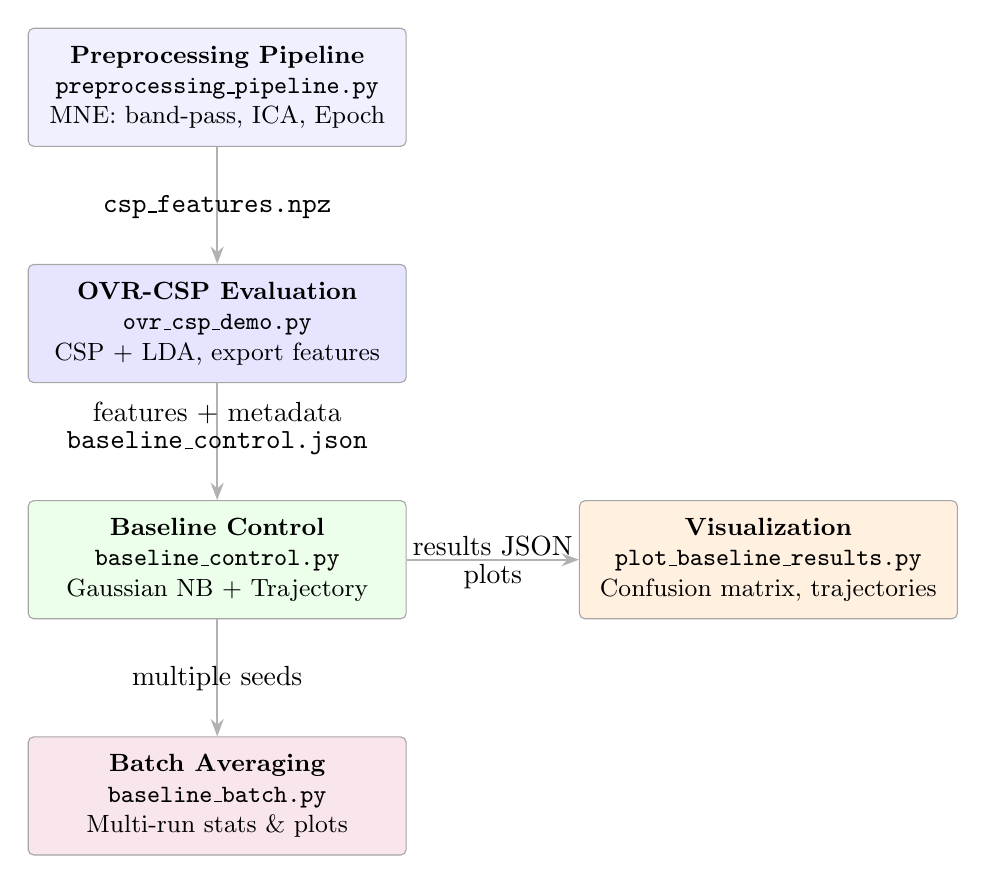
\begin{tikzpicture}[
  node distance=0.6cm,
  >={Stealth[length=2.2mm]},
  flow/.style={->, thick, gray!60},
  basebox/.style={draw=gray!70, rounded corners=2pt, minimum width=48mm,
                  minimum height=15mm, align=center, font=\small, fill=white},
  prebox/.style={basebox, fill=blue!6},
  cspbox/.style={basebox, fill=blue!10},
  ctrlbox/.style={basebox, fill=green!8},
  vizbox/.style={basebox, fill=orange!12},
  batchbox/.style={basebox, fill=purple!10}
]

% Fixed coordinates for a clearer, grid-aligned layout
\node[prebox]  (prep) at (9,0)        {{\bfseries Preprocessing Pipeline}\\\texttt{preprocessing\_pipeline.py}\\MNE: band-pass, ICA, Epoch};
\node[cspbox]  (csp)  at (9,-3)        {{\bfseries OVR-CSP Evaluation}\\\texttt{ovr\_csp\_demo.py}\\CSP + LDA, export features};
\node[ctrlbox] (baseline) at (9,-6) {{\bfseries Baseline Control}\\\texttt{baseline\_control.py}\\Gaussian NB + Trajectory};
\node[vizbox]  (viz)  at (16,-6) {{\bfseries Visualization}\\\texttt{plot\_baseline\_results.py}\\Confusion matrix, trajectories};
\node[batchbox] (batch) at (9,-9)  {{\bfseries Batch Averaging}\\\texttt{baseline\_batch.py}\\Multi-run stats \& plots};

% Arrows with well-placed labels
\draw[flow] (prep) -- node[midway, above=-3mm, text=black, font=\normalsize]{\texttt{csp\_features.npz}} (csp);
\draw[flow] (csp) -- node[midway, above=-3mm, text=black, font=\normalsize]{\shortstack{features + metadata\\\texttt{baseline\_control.json}}} (baseline);
\draw[flow] (baseline) -- node[midway, above=-5mm, text=black, font=\normalsize]{\shortstack{results JSON\\plots}} (viz);
\draw[flow] (baseline) -- node[midway, above=-3mm, text=black, font=\normalsize]{multiple seeds} (batch);

\end{tikzpicture}
}%
\end{center}
\end{document}
